\documentclass{beamer}

\usepackage{amsfonts,amsmath}

\title{Spectral Rigid Body Dynamics}
\author{Mikola Lysenko}

\begin{document}

\newcommand{\R}{\mathbb{R}}

\maketitle

\begin{frame}
\frametitle{Overview}
\end{frame}

\begin{frame}
\frametitle{Rigid Body Dynamics}
Limiting case of continuum dynamics where elastic modulus is infinite.

Pros:
\begin{itemize}
\item Pretty accurate at human scales
\item Good for materials which are stiff
\item Efficient kinematic constraints (good for mechanism design)
\end{itemize}

Cons:
\begin{itemize}
\item Inaccurate at extremely small or large scales
\item Bad for materials with low elastic modulus
\item Not always solvable (See: Painleve's paradox)
\end{itemize}

\end{frame}

\begin{frame}
\frametitle{Configuration Space of a Rigid Body}
Must be a Euclidean isometry

\begin{center}
\includegraphics[height=1.4in]{figures/rigid_body.png}
\end{center}

Identified with translation + rotation, (ie $SE(d) \cong SO(d) \ltimes \R^d$)

Tangent space is isomorphic to $\mathfrak{so}(d+1)$


\end{frame}

\begin{frame}
\frametitle{Phase Flow in $SE(d)$}


\end{frame}

\begin{frame}
\frametitle{Lagrangian Mechanics}

Rephrases the evolution of a physical system in terms of an optimization problem.

\[ \mathcal{L}(q, \dot{q}, t) = T(\dot{q}) - U(q, t) \]

Where
\end{frame}

\end{document}

